\documentclass[12pt]{beamer}

\usepackage[utf8]{inputenc}
\usepackage{url}
\usepackage{natbib}
\usepackage{textcomp}
\usepackage{graphicx}
\graphicspath{{./img/}}

\usepackage{natbib}
\renewcommand{\bibsection}{\subsubsection*{\bibname } }

\setlength\fboxsep{0pt}
\setlength\fboxrule{0.5pt}

\usetheme{Dresden}

\title{Attacks on wireless localization\\ The case of PKES}
\author{Christian Müller}

\section{Introduction}
\subsection*{}
\begin{document}

	\begin{frame}
		\titlepage
	\end{frame}

	\begin{frame}
		\tableofcontents
	\end{frame}

	\begin{frame}
		\frametitle{Terms}
			\begin{description}
				\item[PKE system]\hfill \\
						\textbf{p}assive \textbf{k}eyless \textbf{e}ntry system
				\item[CID] \hfill \\
					\textbf{C}ustomer \textbf{I}dentification \textbf{D}evice
			\end{description}
	\end{frame}
	
\section{Key systems}
\subsection*{}
	\begin{frame}
		\frametitle{Mechanical keys}
		\begin{itemize}
			\onslide<1-2>			
			\item Mechanical key \& lock systems
			\onslide<2-2>
			\item Immobilisers
		\end{itemize}
	\end{frame}
	
	\begin{frame}
		\frametitle{Remote key Systems}
		\begin{itemize}
			\item Button to opens
			\item operate at RF 	%EU 433 MHz
			\item physical key to ignite engine
		\end{itemize}
	\end{frame}

	\begin{frame}
		\frametitle{Passive keyless entry systems}
		\begin{itemize}
			\item car opens when CID is in range
			\item engine can be ignited, if the key is in the car
			\item physical backup key
		\end{itemize}
	\end{frame}

	\begin{frame}
		\frametitle{PKES in detail}
		\begin{enumerate}
			\item Pulling handle transmits a LF-signal
			\item CID wakes up and responds in RF
			\item if response is correct, the vehicle opens
		\end{enumerate}
		\begin{itemize}
			\item same holds for ingiting engine
			\item usually enhanced by RFID
		\end{itemize}
	\end{frame}

\section{Relay attacks}
\subsection*{}
	\begin{frame}
	\frametitle{Introduction}
		\begin{itemize}
			\item relocating signal emission \& reception
			\item underlying problem: proper localization in wireless networks
			\item circumvents higher level authentication
		\end{itemize}
	\end{frame}
	
	\begin{frame}
	\frametitle{Relay over the cable}
		\begin{center}
			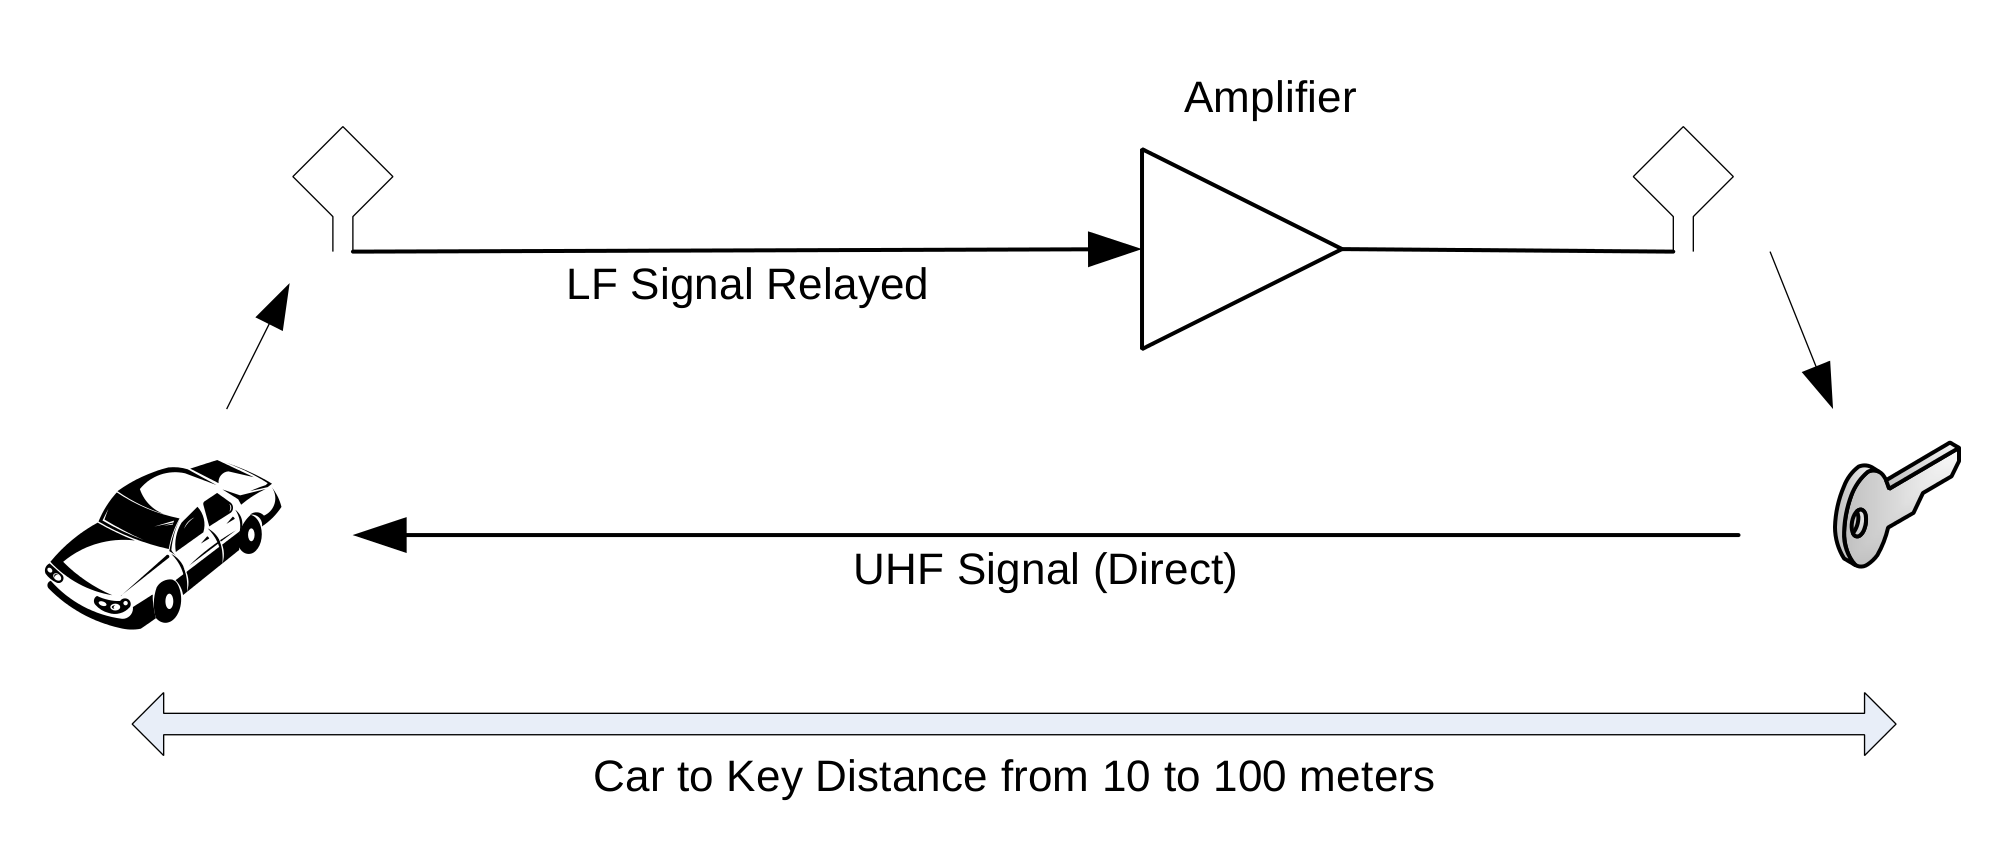
\includegraphics[scale=0.85]{img/franc_relay_over_the_wire.png} 
		\end{center}
	\end{frame}
	
	\begin{frame}
		\frametitle{Relay over the wire}
		\begin{center}
			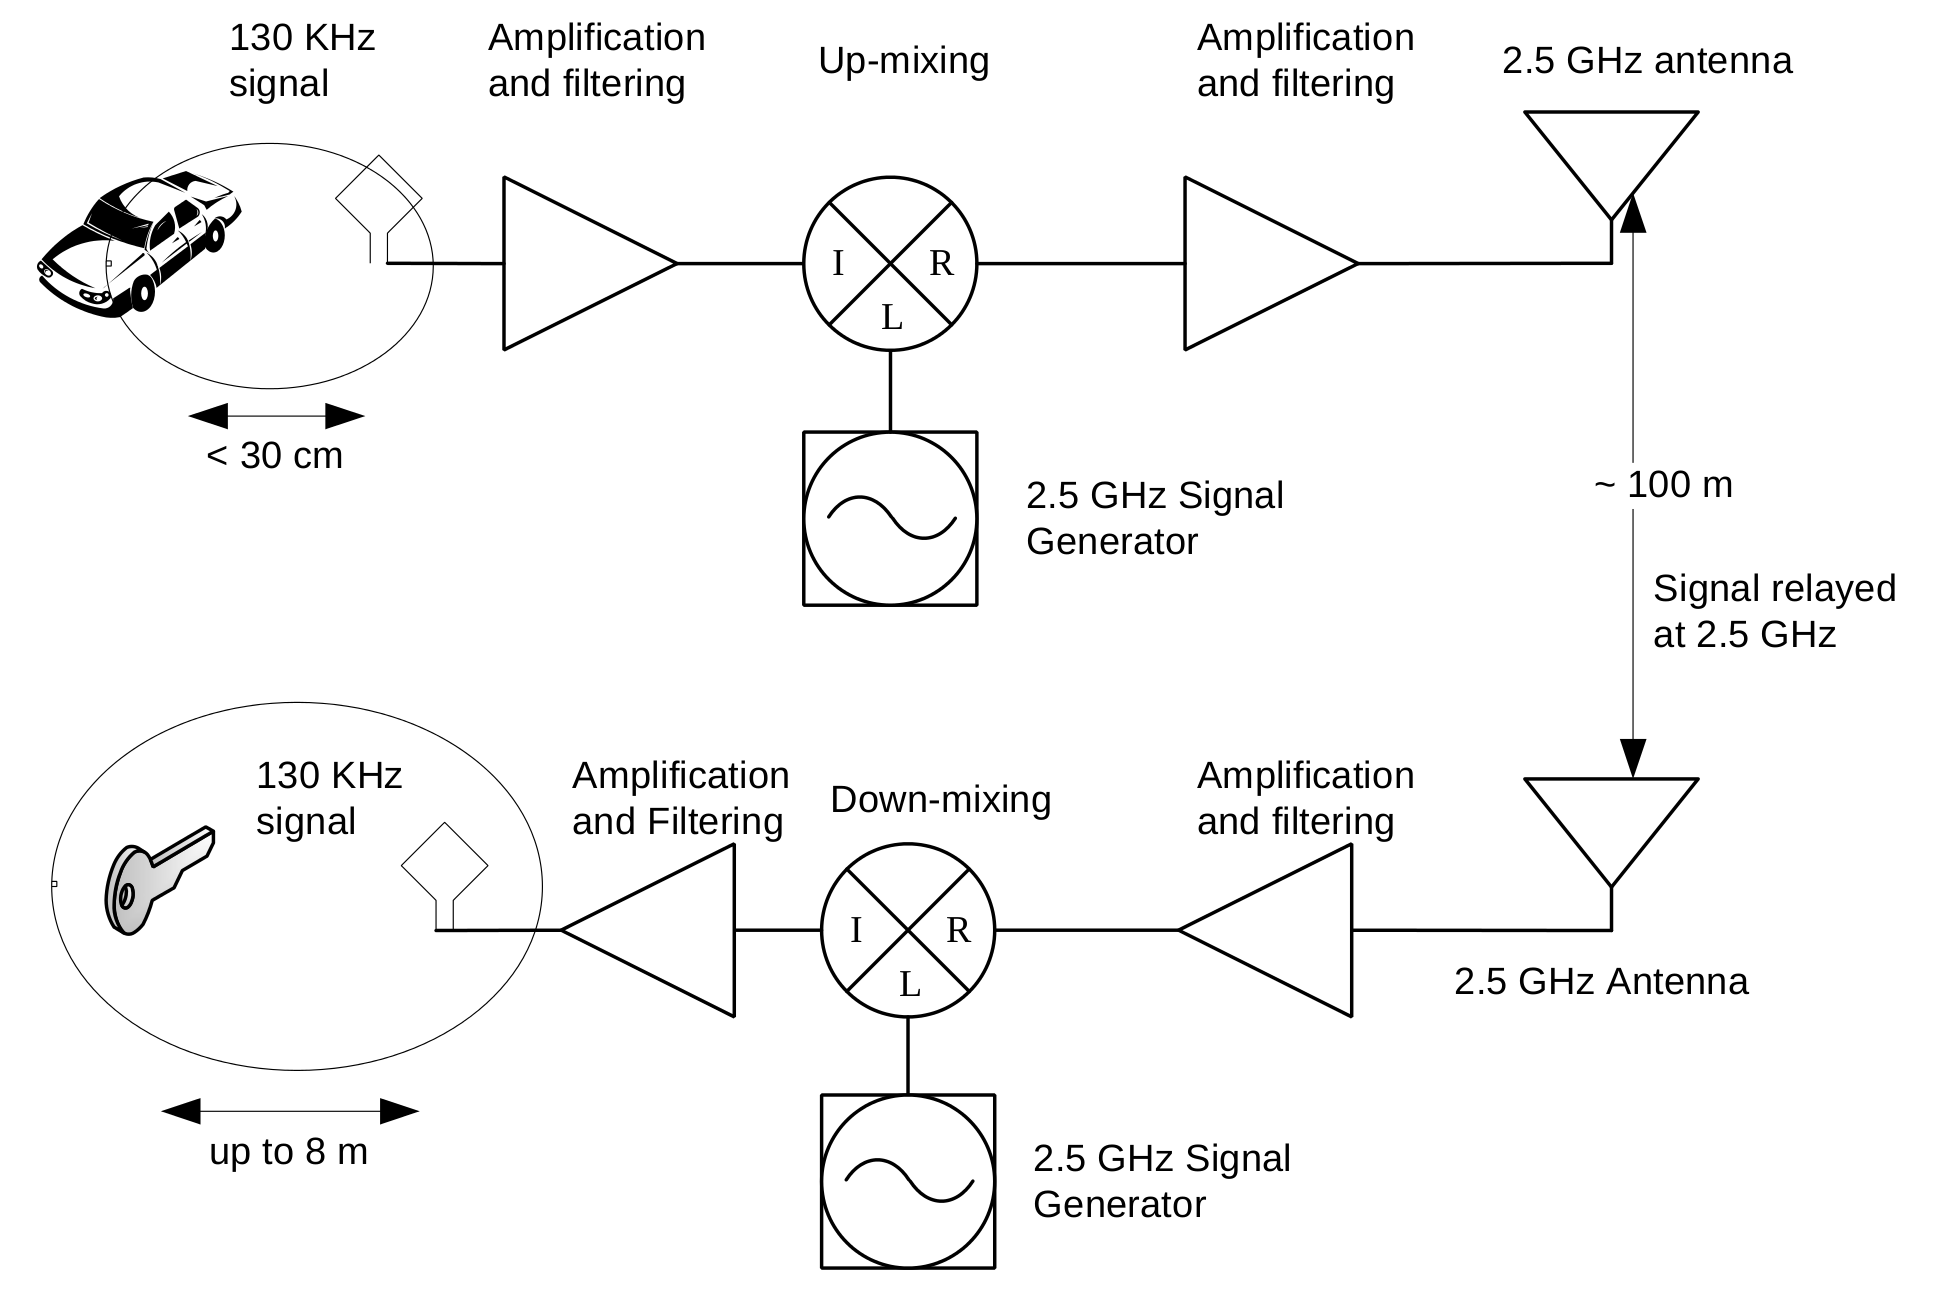
\includegraphics[scale=0.75]{img/franc_relay_over_the_air.png} 	
		\end{center}
	\end{frame}

	\begin{frame}
		\frametitle{This works in practice}
		\begin{itemize}
			\item simple \& inexpensive
			\item tested by \citet*{relayAttacksFranc}
			\item all ten systems vulnerable
		\end{itemize}
	\end{frame}

	\begin{frame}
		\frametitle{Scenario}
		\begin{itemize}
			\item Supermarket
			\item Office
		\end{itemize}
	\end{frame}

\section{Solutions}
\subsection*{}
	\begin{frame}
		\frametitle{}
		\begin{description}
			\item[short term] \hfill \\
				fall back to mechanical keys
			\item[long term] \hfill \\
					different frequencies \\
					distance bounding protocols
		\end{description}
	\end{frame}

	\begin{frame}
		\frametitle{two frequencies}
			\begin{itemize}
				\item use two frequencies
				\item makes relaying more difficult %TODO because..
				\item alternative: seperate commuication channels
			\end{itemize}
	\end{frame}

	\begin{frame}
		\frametitle{Distance bounding}
			\begin{itemize}
				\item be quick
				\item be strict on timing
				\item requires fast hardware
			\end{itemize}
	\end{frame}

\section{Summary \& Literature}
\subsection*{}
	\begin{frame}
		\frametitle{foo}
		bar
	\end{frame}
	\begin{frame}
		%TODO fix size
	\frametitle{Literature}
	\tiny
	\nocite{*}
		\def\newblock{}
		\bibliographystyle{apalike}
		\bibliography{presentation}
	\end{frame}

	\begin{frame}
		\frametitle{Thank you!}
		\begin{center}
			Thank you for your attention!
		\end{center}
	\end{frame}	

\end{document}
\end{input}
